\documentclass[17pt]{beamer}
\usetheme{Singapore}

\usepackage{xcolor}
\usepackage{listings}
\usepackage{courier}
\usepackage{graphicx}

\definecolor{mGreen}{rgb}{0,0.6,0}
\definecolor{mGray}{rgb}{0.5,0.5,0.5}
\definecolor{mPurple}{rgb}{0.8,0,0.82}
\definecolor{backgroundColour}{rgb}{0.95,0.95,0.92}

\lstdefinestyle{CStyle}{
    backgroundcolor=\color{backgroundColour},   
    commentstyle=\color{mGreen},
    keywordstyle=\color{magenta},
    numberstyle=\tiny\color{mGray},
    stringstyle=\color{mPurple},
    basicstyle=\footnotesize,
    breakatwhitespace=false,         
    breaklines=true,                 
    captionpos=b,                    
    keepspaces=true,                 
    numbers=left,                    
    numbersep=5pt,                  
    showspaces=false,                
    showstringspaces=false,
    showtabs=false,                  
    tabsize=2,
    language=C
}

\lstset{basicstyle=\footnotesize\ttfamily,breaklines=true}
\lstset{framextopmargin=50pt,frame=bottomline}

\title{ENGG1003 - Friday Week 1}
\subtitle{Algorithms and Pseudocode}
\author{Brenton Schulz}
\institute{University of Newcastle}
\date{\today}

\begin{document}
\titlepage

\begin{frame}[fragile]
\frametitle{Example frame}
\begin{itemize}
\item thing one
\begin{itemize}
\item subitem
\end{itemize}
\item thing two
\end{itemize}

\begin{lstlisting}[style=CStyle]
#include <stdio.h>
int main() {
	// A comment
	printf("asdf\n");
	return 0;
}
\end{lstlisting}

\end{frame}

\begin{frame}
\frametitle{Columns}
\begin{columns}
\column{1.5in}
left side
\column{1.5in}
right side
\begin{figure}
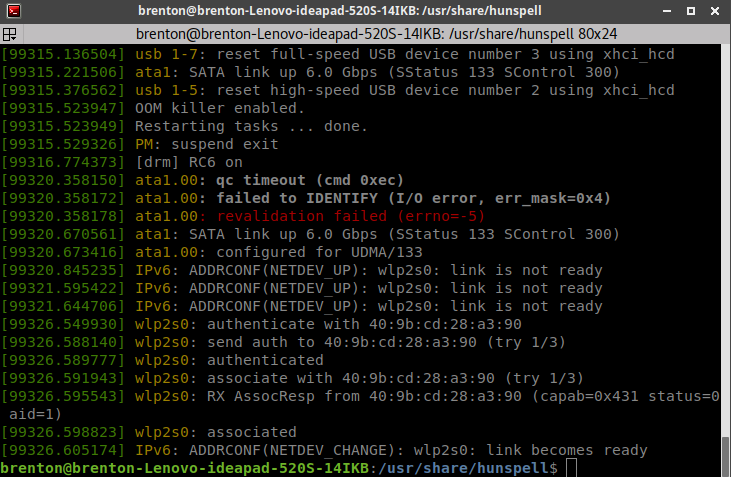
\includegraphics[scale=0.2]{test}
\end{figure}
\end{columns}
\end{frame}

\end{document}